\documentclass[10pt]{paper}
\usepackage{bm,amsmath,graphicx,chngcntr,subfigure}
\usepackage[margin=0.5in]{geometry}
\pagestyle{empty}
\counterwithin{figure}{section}
\pagenumbering{gobble}
\title{Regressions And Stuff}


\begin{document}

\maketitle
\section{Introduction}

In this paper, we discuss various methods of calculating regression. First, we discuss the benfits of using Stochastic Gradient Descent versus Batch Gradient Descent. Next, we analyze the performance of these methods in performing a Least Squares Linear regression. Finally, we discuss blah blah

\section{Gradient Descent}

\emph{Gradient descent} is an iterative optimization algorithm; in other words, it calculates the parameters $\mathbf{x}$ that minimize a given objective function $f(\mathbf{x})$. The algorithm repeatedly translates an initial \emph{guess} $\mathbf{x}_0$ in a direction proportional to the negative \emph{gradient} $\nabla f(x)$.

In every step of the itreration, we update our guess as following:
\begin{align*}
\mathbf{x}_{n+1} = \mathbf{x} - \lambda \nabla f(\mathbf{x}_{n})
\end{align*}
where $\lambda$ is the \emph{step size} of the iteration. The algorithm terminates upon the following convergence condition: 
\begin{align*}
|f(\mathbf{x}_{n+1}) - f(\mathbf{x}_{n})| < \delta
\end{align*}
where $\delta$ is the convergence \emph{threshold}. Upon convergence, the algorithm returns a final guess of $\mathbf{x}_{\text{opt}} = \mathbf{x}_{n+1}$.

In this section, we compare two methods of gradient descent: \emph{batch gradient descent}, which computes a gradient over all samples for each iteration, and \emph{stochastic gradient descent}, which instead uses pointwise gradients.

To analyze the perforamnce of the different algorithms, we use the \emph{Gaussian function}:
\begin{align*}
f(x) = - \dfrac{1}{\sqrt{(2\pi)^n |\Sigma|}} \exp \left[-\dfrac{1}{2} (x - u)^T \Sigma^{-1} (x-u)\right]
\end{align*}
In addition, we use the \emph{quadratic bowl function}:
\begin{align*}
f(x) = \dfrac{1}{2} x^T A x - x^T b 
\end{align*}
Finally, we use the \emph{least squares error} function:
\begin{align*}
J(\theta) = |X\theta - y|^2
\end{align*}


\subsection{Batch Gradient Descent}

In batch gradient descent, for every iteration we calculate the gradient across the entire sample set. In this section, we analyze the affects of step size ($\lambda$), threshold ($\delta$), and initial guess $\mathbf{x}_{0}$ on the performance and accuracy of the gradient descent algorithm. 

First, we note that step size has a significant impact on the convergence rate of the algorithm. We run gradient descent on an arbitrary quadratic bowl function. As we increase the value of $\lambda$ from $0.0001$ to $0.001$, the magnitude of the gradient decreases more quickly, and the algorithm converges faster. Note that in this figure, all of the gradient descents were run with a fixed size of 2000 iterations to illustrate the effects on the gradient over time.


In addition, the step size and threshold control the accuracy of the gradient descent. As step size decreases, we expect a less accurate result because the gradient descent will likely converge at the boundary of the threshold, which a larger step size might lead to convergence well past the threshold. In addition, as the threshold decreases, we expect a more accurate result because the algorithm needs to run for longer before reaching a stable equilibrium. To verify these claims, we run gradient descent using a two-dimensional Gaussian with mean $(10, 10)$. As we vary $\lambda$ and $\delta$, we plot the least-squares error between the returned value and the actual optimum of $(10, 10)$ (see Figure 2). Indeed, the error decreases as $\lambda$ increases and $\delta$ decreases.

Finally, we observe the affect of the initial case on the rate of convergence. When running gradient descent on a two-dimensional Gaussian with mean $(10, 10)$, one would expect that as the intial guess appraoches the optimal value, the convergence rate increases. Indeed, running the algorithm with $\lambda = 1000$ and $\delta = 10^{-11}$, we notice that the rate of convergence is much higher as the initial guess approaches the actual value (see Figure 3). 

\begin{figure}[ht!]
  \centering
  \begin{subfigure}
    \centering
      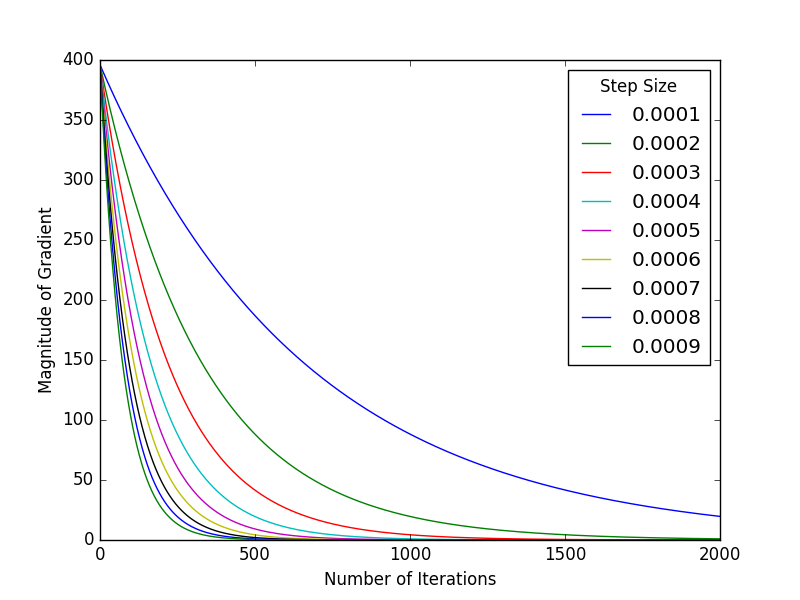
\includegraphics[width=0.3\textwidth]{../images/quadratic_steps_vs_mag}
    % \caption{As the step size increases, the algorithm converges quicker.}
  \end{subfigure}
  \begin{subfigure}
    \centering
      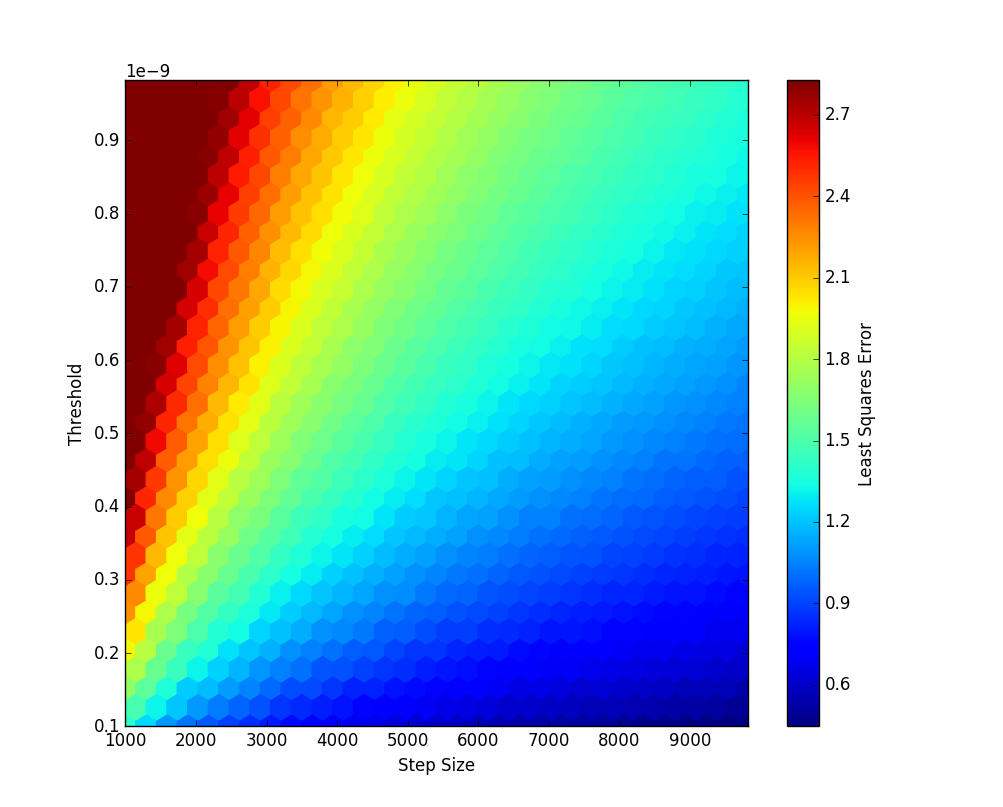
\includegraphics[width=0.3\textwidth]{../images/lsq_error_gradient}
    % \caption{As $\lambda$ increases and $\delta$ decreases, error decreases.}
  \end{subfigure}
  \begin{subfigure}
    \centering
      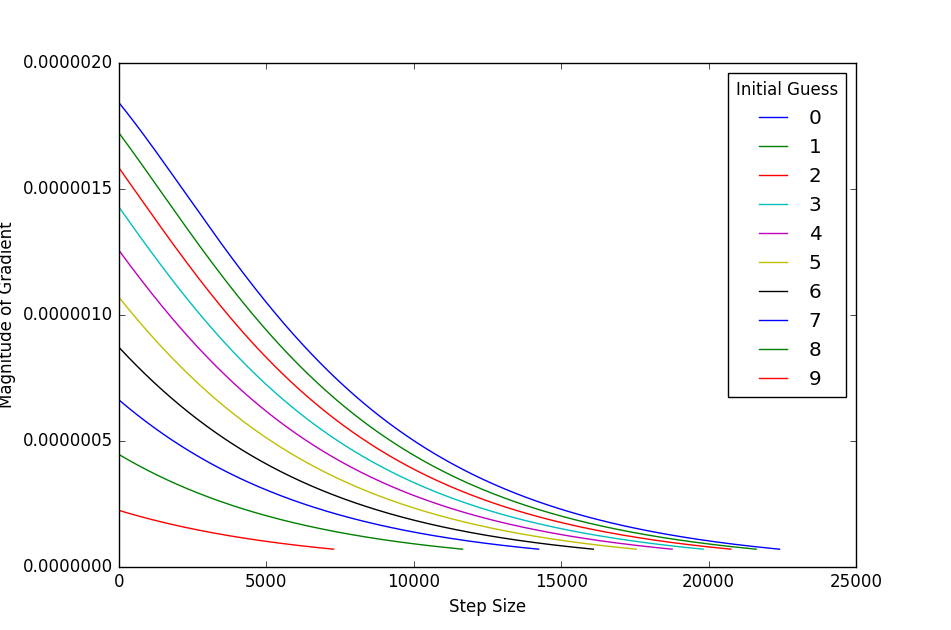
\includegraphics[width=0.3\textwidth]{../images/guess_vs_mags_2}
    % \caption{As $\mathbf{x}_0$ approaches $(10, 10)$, the rate of convergence increases.}
  \end{subfigure}
\end{figure}

\subsection{Stochastic Gradient Descent}

Sometimes, it might be inefficient to compute a gradient over the entire dataset for every iteration, especially when the dataset is large. One way to address this is to use stochastic gradient descent, which uses a pointwise gradient instead. In this experiment, we use least-squares regression, which has a pointwise gradient of 

\begin{align*}
J(\theta; x^{(i)}, y^{(i)}) = (x^{(i)}\theta_t - y^{(i)})^2
\end{align*}
On each iteration, we update our value as follows:
\begin{align*}
\theta_{t+1} = \theta_{t} - \nu_t \nabla_\theta J(\theta_t; x^{(i)}, y^{(i)})
\end{align*}
where $\nabla = (\tau_0 + t)^{-\kappa}$ is the \emph{learning rate}, and $\tau_0$ and $\kappa$ are constants.

The benefit of stochastic gradient descent is that computations are quicker, and thus the algorithm converges faster, with respect to both time and the number of iterations. However, this comes with a decrease in performance, because each iteration uses less information. Refer to Figure 4 for the difference in the magnitude in the gradient between the two methods: note that stochastic gradient descent is much noisier, and in the end, does not converge to as accurate of a value as batch gradient descent does.

\begin{figure}[ht!]
  \center
  \begin{subfigure}
    \centering
      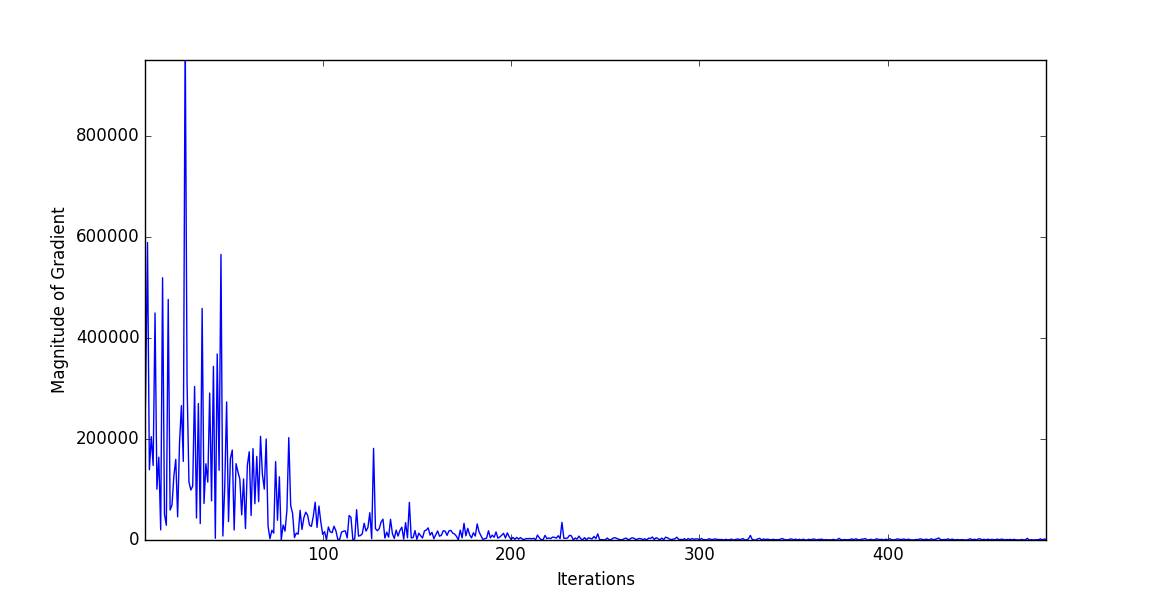
\includegraphics[width=0.45\textwidth]{../images/stochastic_gradient_steps}
    % \caption{Compare to batch gradient descent, the magnitude of the gradient during stochastic gradient descent shows significant noise.}
  \end{subfigure}
  \begin{subfigure}
    \centering
      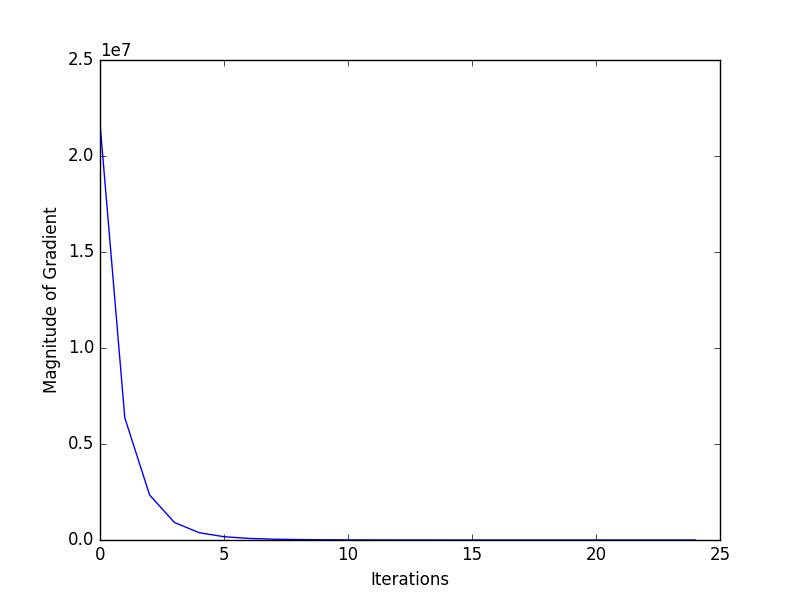
\includegraphics[width=0.45\textwidth]{../images/batch_gradient_steps}
    % \caption{The magnitude of the gradient during batch gradient descent is much smoother.}
  \end{subfigure}
\end{figure}

\subsection{Effect of Finite Gradient}

When the objective function doesn't have a closed form solution, one can approximate the gradient using a central finite difference. In other words, we have 
\begin{align*}
\nabla f(x) \approx \nabla_h[f](x) = \dfrac{f(x+h/2) - f(x-h/2)}{h}
\end{align*}
Therefore, we only need the objective function to approximate the gradient. Note that as $h$ approaches zero, this approaches the actual value of the gradient; and has $h$ approaches infinity this value diverges. Figures 4 and 5 illustrate the impact of $h$ on the accuracy of the gradient: even for relatively large $h$ (especially for the quadratic bowl), the approximation is accurate to several orders of magnitude.

\begin{figure}[ht!]
  \centering
  \begin{subfigure}
    \centering
      \begin{tabular}{c | c}
      $h$  & $\nabla_h[f](x)$ \\  \hline
    0.01 & $-3.1704 \cdot 10^{-7}$ \\
    0.1 & $-3.1704 \cdot 10^{-7}$ \\
    1.0 & $-3.1696 \cdot 10^{-7}$ \\
    10.0 & $-3.0923 \cdot 10^{-7}$ \\
    100.0 & $-2.6198 \cdot 10^{-8}$ \\
    1000.0 & $\approx 0$ \\
      \end{tabular}
    % \caption{As $h$ increases, the accuracy of the central finite difference for this Gaussian decreases. The actual gradient value is $-3.1704 \cdot 10^{-7}$.}
  \end{subfigure}
  \qquad
  \begin{subfigure}
    \centering
      \begin{tabular}{c | c}
      $h$  & $\nabla_h[f](x)$ \\  \hline
    $10^{9}$ & $-280.000000$ \\
    $10^{11}$ & $-279.999991$ \\
    $10^{13}$ & $-280.000944$ \\
    $10^{15}$ & $-280.349077$ \\
    $10^{17}$ & $-299.759591$ \\
    $10^{19}$ & $\approx 0$ \\
      \end{tabular}
    % \caption{As $h$ increases, the accuracy of the central finite difference for this quadratic bowl decreases very slowly. The actual gradient value is $-280$.}
  \end{subfigure}
\end{figure}



\section{Function Basis}
Consider a basic prediction problem where given an input, $x$, we wish to predict a value $y$ (e.g. predict income given GPA, or predict crime rate given temperature). We train on a sample of labeled data (a set of $(x,y)$ pairs) to find a function $f(x)$ that will give the expected $y$ for new inputs $x$.

One approach to this problem is to model $f$ as the linear combination of \emph{basis functions}. In other words, we manually choose functions $\phi_1(x), \dots, \phi_n(x)$ and algorithmically pick coefficients $c_1, \dots, c_n$, which we put together as
\begin{align*}bm
f(x) &= c_1 \phi_1(x) + \dots + c_n \phi_n(x).
\end{align*}
We can rewrite this with 
\begin{align*}
\bm{c} &= \begin{bmatrix} c_1 & \cdots & c_n \end{bmatrix} \\
\bm{\phi}(x) &= \begin{bmatrix} \phi_1(x) & \cdots & \phi_n(x) \end{bmatrix}
\end{align*}
so that 
\begin{align}
f(x) &= \bm{c} \cdot \bm{\phi}(x). \label{eq:predictor}
\end{align}

The choice of the basis functions is somewhat arbitrary and often depends on the problem domain. Common choices are monomials ($\phi_i(x) = x^i$) and sinusoidals ($\phi_i(x) = \sin(i \pi x)$).

As for the algorithm to pick the coefficient vector $\bm{c}$, we discuss three methods: \emph{linear regression}, \emph{ridge regression}, and \emph{LASSO} (least absolute shrinkage and selection operator). We devote one section to exploring each method in the next three sections.

Before moving on, we develop common notation to set up the algorithmic problem. Suppose we are given the training data as column vectors $\bm{x}$ and $\bm{y}$ of length $m$ and have chosen $n$ basis functions given by $\bm{\phi}$. We let $X = \bm{\phi}(\bm{x})$ be the $m$ by $n$ matrix where the $i$-th row is $\bm{\phi}(x_i)$ and $x_i$ is the $i$-th element of $\bm{x}$. Thus, we can roughly frame our algorithm's goal as finding a column vector $\bm{c}$ of size $n$ such that
\begin{align}
\bm{y} &\approx X \bm{c}, \label{eq:problem}
\end{align}
where $X$ and $\bm{y}$ are taken as inputs.

\section{Linear Regression}

Linear regression is a regression method that simply aims to minimize the square of the magnitude of the difference of the two sides of (\ref{eq:problem}):
\begin{align}
\left| \bm{y} - X \bm{c} \right|^2. \label{eq:sse}
\end{align}
The expression in (\ref{eq:sse}) is known as the \emph{sum of squares error}, or SSE, as it is the sum of the squares of the differences in predicted versus real $y$ values. 

One way to find the optimal $\bm{c}$ is to expand the expression and set its partial derivative with respect to $\bm{c}$ equal to zero. Doing so yields
\begin{align}
\bm{c} &= \left( X^T X \right)^{-1} X^T \bm{y}. \label{eq:linearclosed}
\end{align}
We refer to (\ref{eq:linearclosed}) as the closed form for $\bm{c}$.

Another way to find $\bm{c}$ is to perform gradient descent with SSE as the objective function of $\bm{c}$.

We will illustrate and contrast these methods with an example, and then show the effects of choosing a different function basis. Our example is generated by taking $\bm{x}$ as numbers from 0 to 1 at intervals of $0.1$ and 
\begin{align*}
\bm{y} &= \cos(\pi \bm{x}) + \cos(2 \pi \bm{x}) + \text{noise}.
\end{align*}

\subsection{Polynomials with Closed Form}

We use $\bm{\phi}$ of size $n+1$ whose components are monomials of order 0 through $n$ as our funciton basis. Using this to compute $X$ and evaluate the closed form, we can obtain $\bm{c}$. We view the results as a plot of the training data points, the generating curve (without noise), and the predictor $f(x) = \bm{c} \cdot \bm{\phi}(x)$. This is shown in Figure \ref{fig:poly} for several values of $n$.

\begin{figure}[ht!]
  \centering
  \label{fig:poly}
  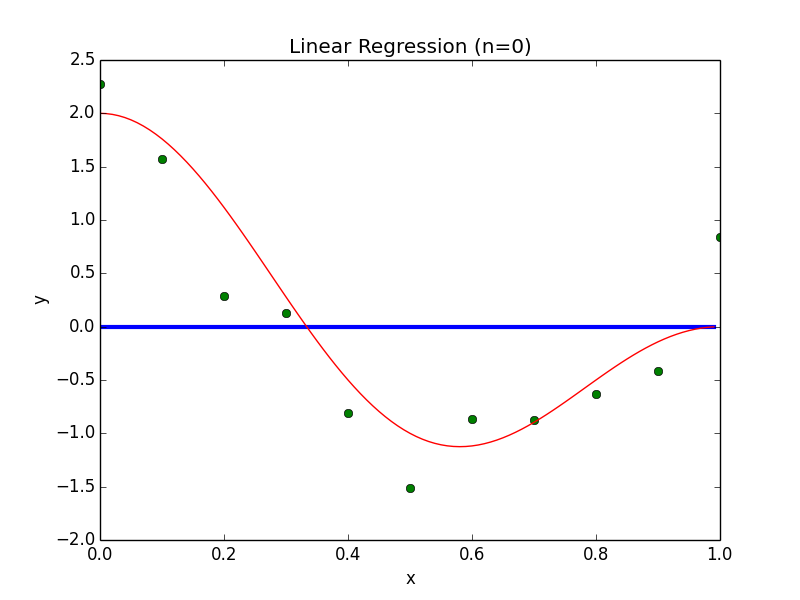
\includegraphics[width=0.24\textwidth]{../images/poly0.png}
  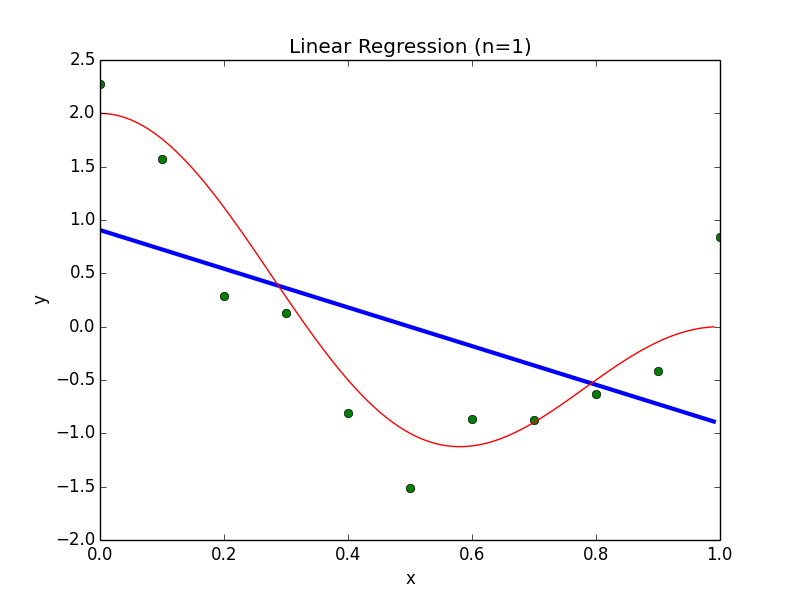
\includegraphics[width=0.24\textwidth]{../images/poly1.png}
  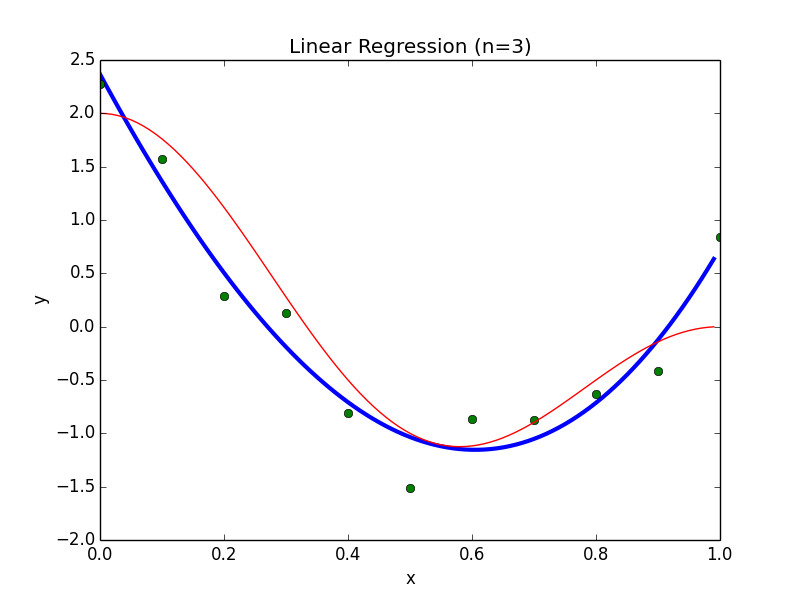
\includegraphics[width=0.24\textwidth]{../images/poly3.png}
  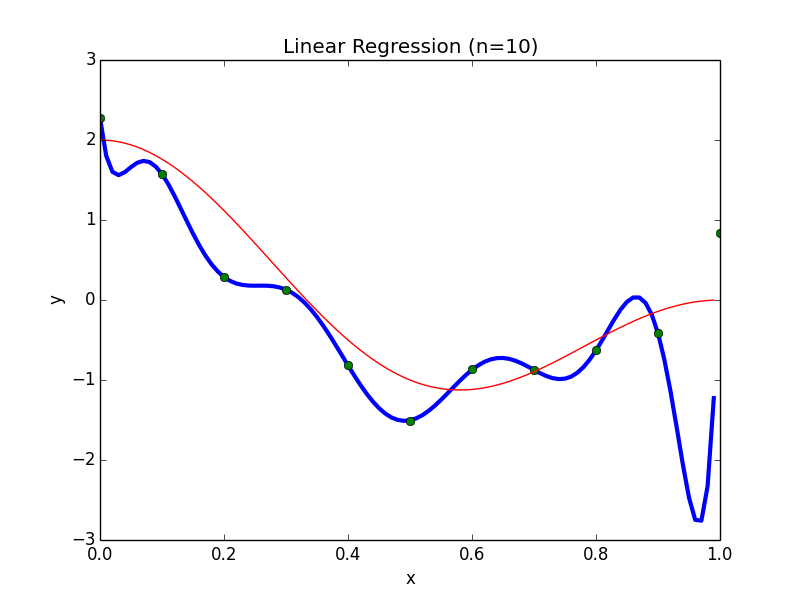
\includegraphics[width=0.24\textwidth]{../images/poly10.png}
  \caption{Training data (green), generating curve (red), and predicted curve (blue) for $n = 0, 1, 3, 10$.}
\end{figure}

We can see that increasing the dimension of the function basis improves the training accuracy of our predictor.

\subsection{Polynomials with Gradient Descent}

Use batch gradient descent on the SSE function on some values of M. Describe your experience
with initial guesses, step sizes and convergence thresholds. Compare with using SGD on the
same data. Explain your results in terms of the properties of the function being optimized and
the properties of the algorithms.

\subsection{Cosines with Closed Form and Gradient Descent}

We now try using the function basis consisting of $\cos(\pi x), \cos(2 \pi x), \dots, \cos(n \pi x)$. In this case the closed form and both versions of gradient descent all give the same coefficient vectors after converging. We plot in Figure \ref{fig:cos} comparisons for a couple values of $n$.

\begin{figure}[ht!]
  \centering
  \label{fig:cos}
  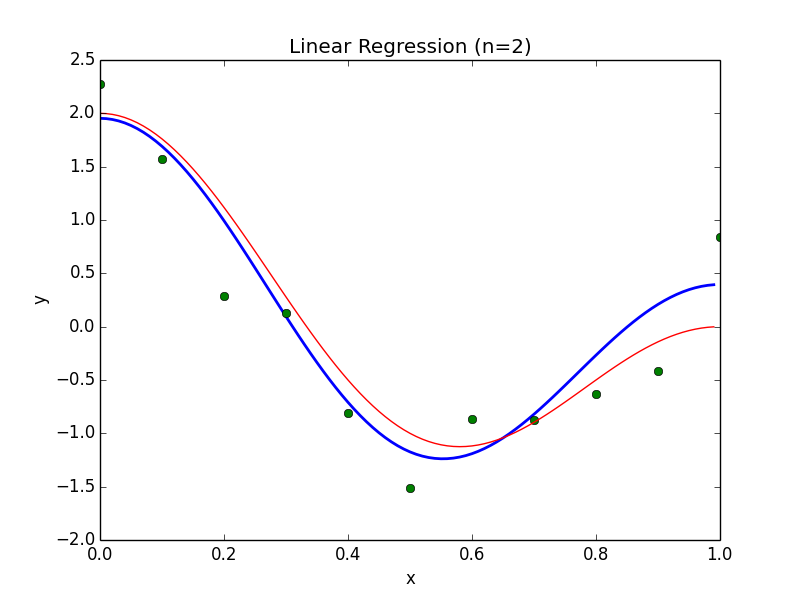
\includegraphics[width=0.3\textwidth]{../images/cos2.png}
  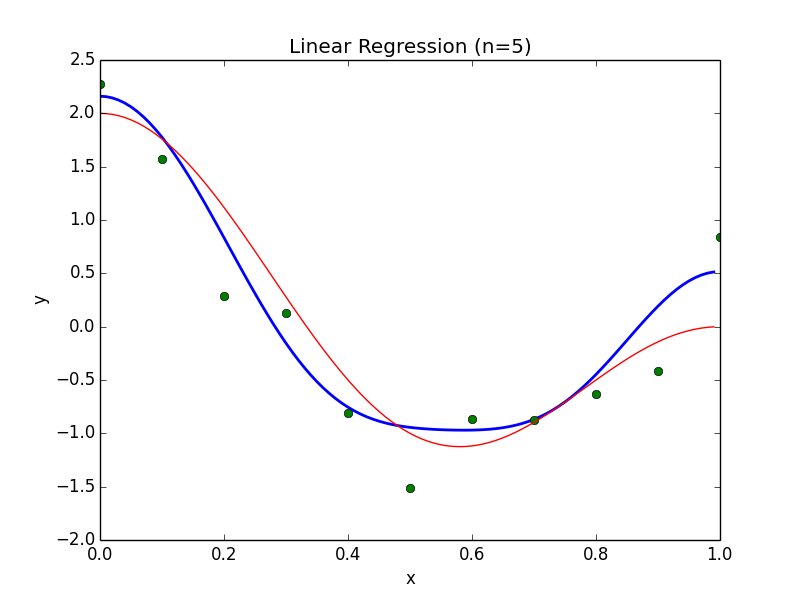
\includegraphics[width=0.3\textwidth]{../images/cos5.png}
  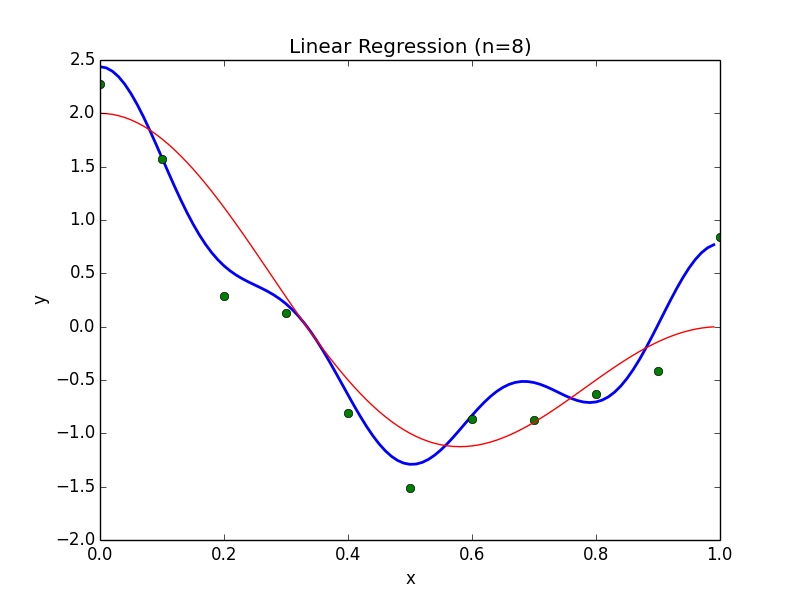
\includegraphics[width=0.3\textwidth]{../images/cos8.png}
  \caption{Training data (green), generating curve (red), and predicted curve (blue) for $n=2, 5, 8$.}
\end{figure}

A notable observation is that even when the same basis functions were used as in the generating function ($\cos(\pi x)$ and $\cos(2\pi x)$ when $n=2$), we obtained a slightly different predicted curve. This is due to the added noise.

Also, when we increase the dimension of the basis ($n=8$) the predicted curve becomes more complex. Although it is more accurate for the training data, it is more sensitive to the noise and so wouldn't generalize well to new test data. This behavior is called \emph{overfitting}, which results when the coefficients become too large or when too many features (basis functions) are used. We will see below that these issues can be addressed using ridge regression and LASSO, respectively.

\section{Ridge Regression}

Ridge regression is similar to linear regression in that its choice of $\bm{c}$ aims to minimize SSE, but in addition also aims to minimize the size of the coefficients themselves. Tangibly, this is achieved by choosing $\bm{c}$ that gives the minimal value of
\begin{align}
\left| \bm{y} - X \bm{c} \right|^2 + \lambda \left| \bm{c} \right|^2. \label{eq:ridgeobjective}
\end{align}
We can tune the sensitivity to coefficient sizes by adjusting the parameter $\lambda$. At the extreme, $\lambda = 0$ will have no consideration of coefficient size and will be the same as linear regression.

Again, there are two ways to arrive at the desired $\bm{c}$ from here. First, we can expand (\ref{eq:ridgeobjective}) and set the partial derivative with respect to $\bm{c}$ equal to zero, which gives
\begin{align*}
\bm{c} &= \left( X^T X + \lambda I \right)^{-1} X^T \bm{y}. \label{eq:ridgeclosed}
\end{align*}
Second, we can perform gradient descent and converge to the optimal value of $\bm{c}$ numerically.

In general, the advantage of the second term in the objective function is that resulting coefficients are smaller, thus empirically less sensitive to noise and more accurate on unseen data.

\subsection{Continuation of Simple Example}

In this subsection we apply ridge regression to the same example as the previous section, in which linear regression showed some overfitting. Varying $\lambda$ and $n$ gives us the plots in Figure \ref{fig:ridge}.

\begin{figure}[ht!]
  \centering
  \label{fig:ridge}
  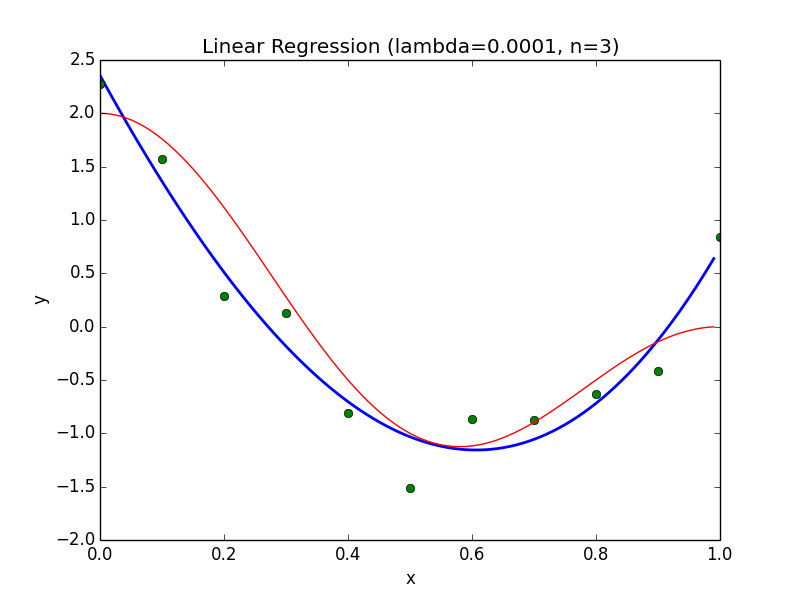
\includegraphics[width=0.24\textwidth]{../images/ridge3low.png}
  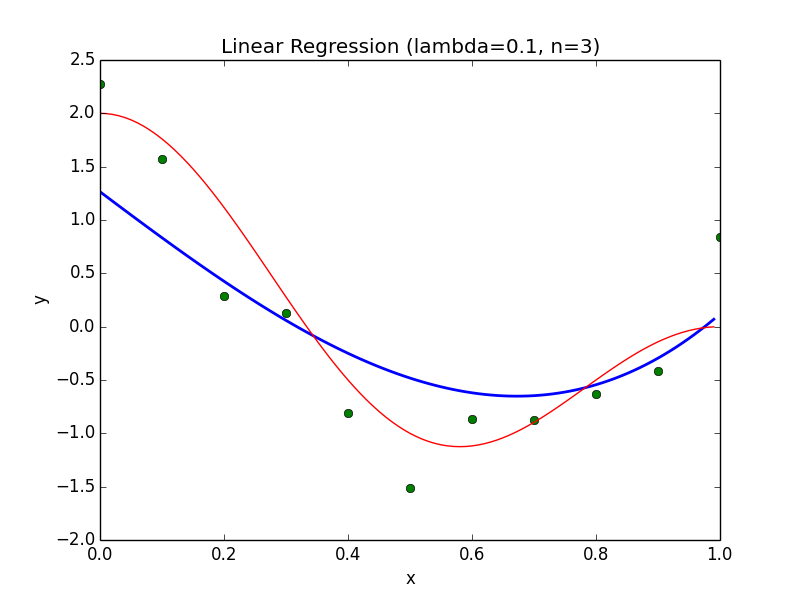
\includegraphics[width=0.24\textwidth]{../images/ridge3high.png}
  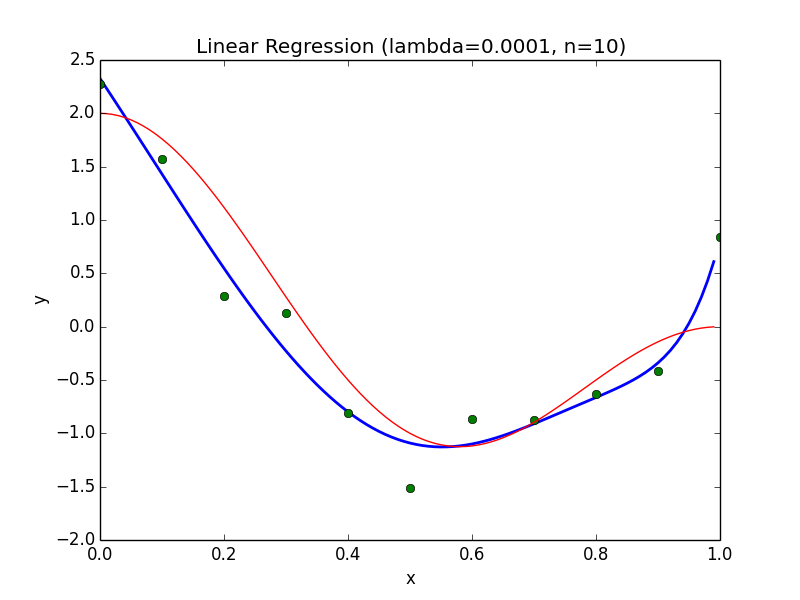
\includegraphics[width=0.24\textwidth]{../images/ridge10low.png}
  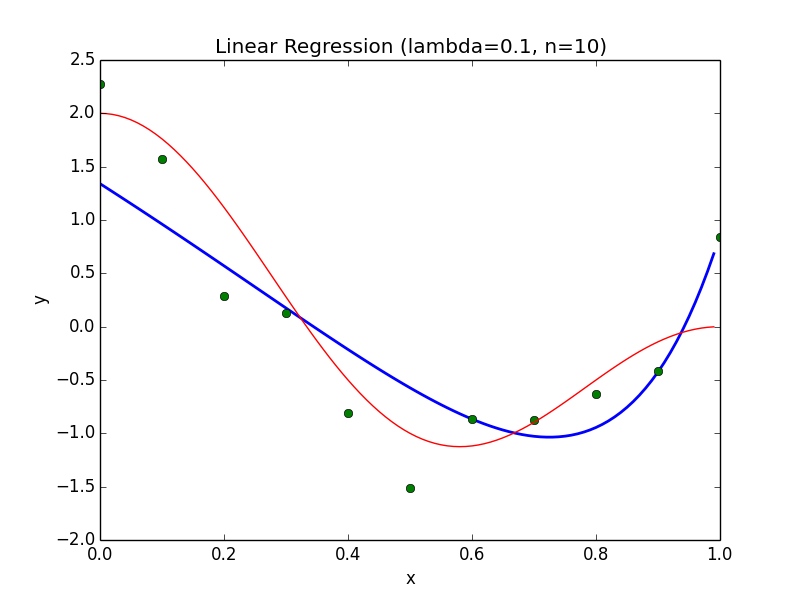
\includegraphics[width=0.24\textwidth]{../images/ridge10high.png}
  \caption{Training data (green), generating curve (red), and predicted curve (blue) for $\lambda=0.0001, 0.1$ and $n = 3, 10$.}
\end{figure}

We can see that a good value of $\lambda$ gives a decent fit, while $\lambda$ too large results in \emph{underfitting}, where the prediction is not sensitive enough to the training data.

\subsection{Training and Validation}

As we just illustrated, choosing a good value of $\lambda$ is crucial for generalizing well. We now present a process for finding a good value for $\lambda$ (as well as $n$). Such a process is called \emph{model selection}.

We divide the given labeled data into two groups, one called the training set and one called the validation set. We vary $n$ and $\lambda$, and for each combination we train as above on the training set and compute SSE on the validation set. Finally, we select the combination of parameters that resulted in the smallest validation SSE.

To illustrate in an example, we have three sets of data: set A, set B, and a validation set. We perform the above process twice, once training on A and testing on B, and once vice versa. In both cases we try a variety of values of $\lambda$ and $n$ then evaluate the SSE on the validation set. The results are given in Figure \ref{fig:validationtable}
\begin{figure}[ht!]
  \centering
  \label{fig:validationtable}
  \begin{tabular}{c|cccccc}
    & 1e-05 & 0.0001 & 0.001 & 0.01 & 0.1 \\ \hline
  0 & 62.00 & 62.00 & 62.00 & 62.01 & 62.06 \\
  1 & 2.90 & 2.90 & 2.90 & 2.90 & 2.94 \\
  2 & 2.35 & \textbf{2.35} & 2.35 & 2.36 & 2.43 \\
  3 & 2.37 & 2.37 & 2.37 & 2.39 & 2.55 \\
  4 & 3.58 & 3.58 & 3.58 & 3.59 & 3.67 \\
  5 & 4.14 & 4.14 & 4.14 & 4.12 & 3.97 \\
  6 & 3.98 & 3.98 & 3.98 & 3.96 & 3.89 \\
  7 & 4.07 & 4.07 & 4.06 & 4.03 & 3.89 \\
  \end{tabular}
  \qquad
  \begin{tabular}{c|ccccc}
    & 0 & 0.3 & 0.6 & 0.9 & 1.2 \\ \hline
  0 & 72.44 & 70.95 & 69.63 & 68.47 & 67.44 \\
  1 & 35.19 & 34.09 & 33.14 & 32.34 & 31.67 \\
  2 & 38.53 & 38.65 & 38.76 & 38.87 & 38.96 \\
  3 & 30.30 & 28.46 & \textbf{28.09} & 28.47 & 29.21 \\
  4 & 130.20 & 67.54 & 51.63 & 46.17 & 44.35 \\
  5 & 625.43 & 368.40 & 287.26 & 242.74 & 212.14 \\
  6 & 680.05 & 533.60 & 481.26 & 440.20 & 406.68 \\
  7 & 492.85 & 360.39 & 448.42 & 544.91 & 634.85 \\
  \end{tabular}
  \caption{SSE values on validation set after training with various $n$ (rows) and $\lambda$ (columns). Left: training on set A. Right: training on set B. Best values bolded.}
\end{figure}
The SSE for the first case with $n = 2$ and $\lambda = 0.0001$, tested on set B, is $25.752$. In the second case, tested on set A with $n = 3$ and $\lambda = 0.6$, the SSE is $40.087483697$. Testing with parameters $n=4$ and $\lambda = 0.1$ for both cases, which the table would predict to be suboptimal, indeed gives bigger test SSEs of 31.1388659319 and 64.9392925156, respectively.

We can see in this example that the choice of training set matters. Also, we note that the best values for the parameters $n$ and $\lambda$ depends heavily on the given data.


\section{LASSO}



\end{document}

